\section{Inverse Texture Synthesis}
Another algorithm for summarizing images is the \textit{inverse texture synthesis} found by \textsc{Wei, Han, Zhou, Bao, Guo} and \textsc{Shum}.\\
It works similar to bidirectional similarity (see section 2) by comparing for completeness and coherence. Those steps only have different names (forward M-step and inverse M-step) and the algorithm does not use gradual resizing instead the target images changes continously. \\
Inverse texture synthesis brings a user-controlleable feature with it: control maps. So we will first learn about control maps and then introduce the technical details of the algorithm.

\subsection{Control maps}
As mentioned before control maps are a big feature in inverse texture synthesis not only because they are user-controllable. Technically they are an additional layer for computation to manipulate how the final texture will look like similar to importance weights of bidirectional similarity (section 2.3.3).\\
Figure \ref{fig:Control maps} shows an example for control maps. As you can see the control maps 'controls' where the brown spots are located on the final texture. The non-black parts work like a mask to show a desired percentage of the brown spots where white means 100\% brown.\\
If we would change the white parts of the control map, the brown spots on he texture would change too.\\
User can define their own control maps to achieve different textures like painting dirt on a mesh\footnotemark  of a vase. 

\footnotetext{A \textit{mesh} is a collection of polygons in 3D computer graphics representing a 3D object.}

\begin{figure}[h]
\centering
\includegraphics[scale=0.9]{img/controlmaps}
\caption[Control maps]{On the left a texture, on the right the control map for the texture.\\ Images from \cite{its}.}
\label{fig:Control maps}
\end{figure}


\subsection{Algorithm}
\subsubsection{z E-step}
\subsubsection{Forward M-step}
\subsubsection{Inverse M-step}
\subsubsection{w E-step}
\subsection{Orientation fields}
\subsection{Example}
\subsection{Performance and limitations}